\documentclass[12pt]{article}

% Modelo SBC: se o arquivo oficial sbc-template.sty estiver na pasta, ele é usado.
% Caso contrário, um layout equivalente (duas margens, Times) é aplicado.
\IfFileExists{sbc-template.sty}{%
  \usepackage{sbc-template}%
}{%
  \usepackage{times}%
  \usepackage[a4paper,top=3cm,bottom=2.5cm,left=3cm,right=3cm]{geometry}%
}
\usepackage[utf8]{inputenc}
\usepackage[T1]{fontenc}
\IfFileExists{brazilian.ldf}{\usepackage[brazilian]{babel}}{\IfFileExists{portuges.ldf}{\usepackage[brazilian]{babel}}{}}
\usepackage{graphicx}
\usepackage{booktabs}
\usepackage{tikz}
\usepackage{listings}
\usepackage{url}
\usepackage[hidelinks]{hyperref}
\usetikzlibrary{positioning,shapes.geometric,arrows.meta,fit}

\lstset{basicstyle=\ttfamily\footnotesize,breaklines=true,frame=single,
  columns=fullflexible,keepspaces=true,
  literate={á}{{\'a}}1 {ã}{{\~a}}1 {é}{{\'e}}1 {ç}{{\c c}}1 {í}{{\'i}}1 {ó}{{\'o}}1 {ú}{{\'u}}1}

\newcommand{\wf}[1]{\textbf{#1}}

\title{Sistema de Cadastro de Produtos: Front-end Integrado a API Node.js e SQL Server}
\author{Giulia Lavinia Barbosa\\
Pontifícia Universidade Católica de Minas Gerais (PUC Minas)\\
Belo Horizonte -- MG -- Brasil}
\date{}

\begin{document}
\maketitle

\section{Descrição do problema}

Pequenos comércios precisam manter um catálogo de produtos organizado: cadastrar itens, corrigir preços e estoques, remover itens descontinuados e consultar rapidamente quais produtos atendem a determinado critério (por exemplo, itens com estoque baixo ou de uma categoria específica). Quando esse controle é feito em planilhas, surgem códigos duplicados, dados desatualizados e dificuldade de consulta.

Este trabalho apresenta a segunda etapa do projeto: um \textit{front-end} web integrado ao \textit{back-end} desenvolvido na primeira etapa (API REST em Node.js com banco SQL Server). O objetivo é permitir que um usuário execute, por telas, todas as operações da API: cadastro, edição, exclusão e pesquisa com filtros. Todos os dados exibidos vêm do banco de dados por meio da API; não há dados estáticos ou simulados no código do front-end.

\section{Modelagem adotada}

\subsection{Entidade e banco de dados}

O sistema possui a entidade \texttt{Produto}, persistida na tabela \texttt{Produtos} do SQL Server Express por meio do ORM Sequelize (driver \texttt{mssql}). A Tabela~\ref{tab:modelo} descreve os campos. O campo \texttt{codigo} possui restrição de unicidade, e a API rejeita preço ou estoque negativos e avaliação fora do intervalo de 0 a 5.

\begin{table}[ht]
\centering
\caption{Modelo da entidade Produto.}\label{tab:modelo}
\small
\begin{tabular}{llp{5.2cm}}
\toprule
\textbf{Campo} & \textbf{Tipo} & \textbf{Restrições}\\
\midrule
id & INTEGER & Chave primária, autoincremento\\
nome & STRING(120) & Obrigatório\\
codigo & STRING(60) & Obrigatório, único\\
preco & DECIMAL(10,2) & Obrigatório, $\geq 0$\\
descricao & STRING(1000) & Obrigatório\\
quantidadeEstoque & INTEGER & Obrigatório, $\geq 0$\\
avaliacao & DECIMAL(2,1) & Obrigatório, entre 0 e 5\\
categoria & STRING(80) & Obrigatório\\
imagemUrl & STRING(1000) & Opcional\\
createdAt, updatedAt & DATETIME & Gerados automaticamente\\
\bottomrule
\end{tabular}
\end{table}

\subsection{Arquitetura}

A aplicação segue uma arquitetura em três camadas (Figura~\ref{fig:arq}). O navegador executa HTML, CSS (Bootstrap 5) e JavaScript puro; as páginas são servidas pelo próprio Express, que também expõe a API REST. A API acessa o SQL Server via Sequelize.

\begin{figure}[ht]
\centering
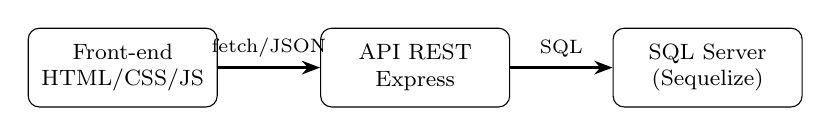
\begin{tikzpicture}[node distance=1.3cm,
  box/.style={draw,rounded corners,minimum width=2.4cm,minimum height=1cm,align=center,font=\footnotesize},
  arr/.style={-{Stealth},thick}]
  \node[box] (fe) {Front-end\\HTML/CSS/JS};
  \node[box,right=of fe] (api) {API REST\\Express};
  \node[box,right=of api] (db) {SQL Server\\(Sequelize)};
  \draw[arr] (fe) -- node[above,font=\scriptsize]{fetch/JSON} (api);
  \draw[arr] (api) -- node[above,font=\scriptsize]{SQL} (db);
\end{tikzpicture}
\caption{Arquitetura em três camadas.}\label{fig:arq}
\end{figure}

\subsection{Rotas da API utilizadas}

A Tabela~\ref{tab:rotas} lista as rotas e a tela que as consome. As rotas \texttt{GET /api/produtos} (com filtros) e \texttt{GET /api/produtos/resumo} foram estendidas nesta etapa para atender às consultas do front-end.

\begin{table}[ht]
\centering
\caption{Rotas da API e telas que as utilizam.}\label{tab:rotas}
\small
\begin{tabular}{llp{3.2cm}}
\toprule
\textbf{Método e rota} & \textbf{Função} & \textbf{Tela}\\
\midrule
POST /api/produtos & Cadastrar & Home e Gerenciar\\
GET /api/produtos?filtros & Listar e filtrar & Home e Gerenciar\\
GET /api/produtos/:id & Detalhar & Detalhes\\
GET /api/produtos/codigo/:codigo & Busca por código & Gerenciar\\
GET /api/produtos/categoria/:cat & Busca por categoria & Consulta de categoria\\
GET /api/produtos/resumo & Agregações & Gerenciar (painel)\\
PUT /api/produtos/:id & Editar & Detalhes e Gerenciar\\
DELETE /api/produtos/:id & Excluir & Detalhes e Gerenciar\\
\bottomrule
\end{tabular}
\end{table}

\section{Wireframes}

Os wireframes de média fidelidade foram elaborados em tons de cinza antes do desenvolvimento. O protótipo completo está disponível em: \url{COLE_AQUI_O_LINK_DO_FIGMA}. A Figura~\ref{fig:wf} resume o esboço das duas telas principais.

\begin{figure}[ht]
\centering
\resizebox{\linewidth}{!}{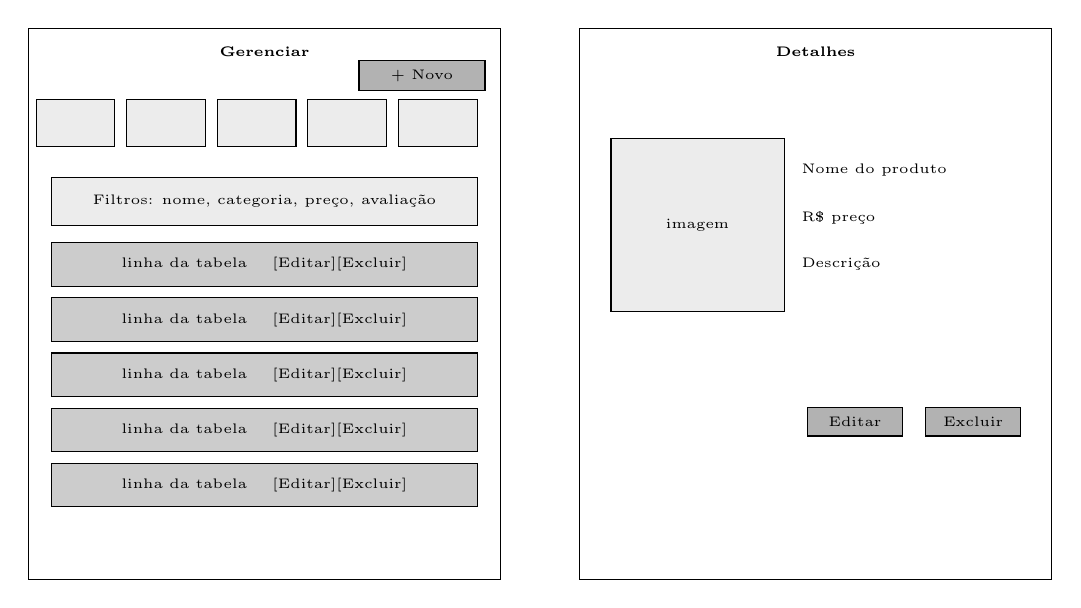
\begin{tikzpicture}[x=0.1cm,y=0.1cm,font=\tiny,
  r/.style={draw,fill=gray!15},
  t/.style={draw,fill=gray!40}]
  % Tela Gerenciar
  \draw (0,0) rectangle (60,70);
  \node at (30,67) {\wf{Gerenciar}};
  \foreach \i in {0,...,4}{\node[r,minimum width=1cm,minimum height=0.6cm] at (6+\i*11.5,58) {};}
  \node[r,minimum width=5.4cm,minimum height=0.6cm] at (30,48) {Filtros: nome, categoria, preço, avaliação};
  \foreach \i in {0,...,4}{\node[t,minimum width=5.4cm,minimum height=0.55cm] at (30,40-\i*7) {linha da tabela \quad [Editar][Excluir]};}
  \node[draw,fill=gray!60,minimum width=1.6cm] at (50,64) {+ Novo};
  % Tela Detalhes
  \draw (70,0) rectangle (130,70);
  \node at (100,67) {\wf{Detalhes}};
  \node[r,minimum width=2.2cm,minimum height=2.2cm] at (85,45) {imagem};
  \node[anchor=west] at (97,52) {Nome do produto};
  \node[anchor=west] at (97,46) {R\$ preço};
  \node[anchor=west] at (97,40) {Descrição};
  \node[draw,fill=gray!60,minimum width=1.2cm] at (105,20) {Editar};
  \node[draw,fill=gray!60,minimum width=1.2cm] at (120,20) {Excluir};
\end{tikzpicture}}
\caption{Esboço dos wireframes (Gerenciar e Detalhes).}\label{fig:wf}
\end{figure}

\section{Telas desenvolvidas}

O front-end foi construído com HTML, CSS, Bootstrap 5 e JavaScript, com três telas.

\begin{description}
\item[Home (\texttt{index.html}).] Carrossel de destaques, cards com os 12 produtos mais recentes e cadastro por modal.
\item[Detalhes (\texttt{detalhes.html}).] Exibe todos os campos do produto, com edição por modal e exclusão com confirmação.
\item[Gerenciar (\texttt{gerenciar.html}).] Tabela com cadastro, edição e exclusão; filtros por nome, categoria, faixa de preço, avaliação mínima e estoque máximo; ordenação; busca por código; e painel de resumo com gráfico por categoria.
\end{description}

% Para inserir capturas de tela, salve-as em relatorio/img/ e descomente:
% \begin{figure}[ht]\centering
% \includegraphics[width=\linewidth]{img/gerenciar.png}
% \caption{Tela Gerenciar com filtros e resumo.}
% \end{figure}

\section{Consultas e resultados no front-end}

\subsection{Consulta 1: filtro combinado (banco e rota)}

Ao preencher, por exemplo, categoria ``Informática'' e preço máximo de R\$ 300,00, o front-end envia:

\begin{lstlisting}
GET /api/produtos?categoria=Informática&precoMax=300&ordem=menorPreco
\end{lstlisting}

A rota monta a cláusula \texttt{WHERE} dinamicamente com o Sequelize, o que equivale a:

\begin{lstlisting}[language=SQL]
SELECT * FROM Produtos
WHERE categoria LIKE 'Informática' AND preco <= 300
ORDER BY preco ASC;
\end{lstlisting}

O resultado é exibido na tabela da tela Gerenciar, com o contador de itens encontrados atualizado. Com os dados fictícios, retornam o mouse sem fio e o teclado mecânico.

\subsection{Consulta 2: painel de resumo (agregação)}

Ao abrir a tela Gerenciar, o front-end chama \texttt{GET /api/produtos/resumo}, que executa consultas agregadas:

\begin{lstlisting}[language=SQL]
SELECT COUNT(id), SUM(quantidadeEstoque),
       SUM(preco * quantidadeEstoque), AVG(avaliacao)
FROM Produtos;

SELECT categoria, COUNT(id), AVG(preco)
FROM Produtos GROUP BY categoria
ORDER BY COUNT(id) DESC;
\end{lstlisting}

Os resultados alimentam os cartões (total de produtos, unidades, valor em estoque, avaliação média, estoque baixo) e o gráfico de barras por categoria.

\subsection{Consulta 3: busca por código}

O campo ``Código exato'' chama \texttt{GET /api/produtos/codigo/INF-001}. Se o código existir, a tabela mostra apenas o produto; caso contrário, a API responde 404 e a tela exibe a mensagem ``Nenhum produto encontrado''.

\section{Artefatos e repositório}

O código-fonte completo, o histórico de commits e as instruções de execução estão no repositório: \url{COLE_AQUI_O_LINK_DO_GITHUB}. O vídeo de apresentação (pitch de 3 a 5 minutos) foi submetido no Canvas.

\paragraph{Como executar.} Criar o banco \texttt{CadastroProdutos} no SQL Server, copiar \texttt{.env.example} para \texttt{.env}, executar \texttt{npm install}, \texttt{npm run seed} e \texttt{npm start}, e acessar \url{http://localhost:3000}.

\end{document}
